\documentclass[tikz,border=8pt]{standalone}
% Shared look for every TikZ diagram. Load with \input{../../tools/tikz-style.tex}
\usepackage[T1]{fontenc}
\usepackage{lmodern}
\renewcommand{\sfdefault}{lmr}  % diagrams use the same serif as the text
\usetikzlibrary{arrows.meta, positioning, shapes.geometric, calc, fit, backgrounds}
\definecolor{cblue}{HTML}{4C78A8}
\definecolor{corange}{HTML}{F58518}
\definecolor{cgreen}{HTML}{54A24B}
\definecolor{cred}{HTML}{E45756}
\definecolor{cpurple}{HTML}{B279A2}
\definecolor{cgrey}{HTML}{6B6B6B}
\tikzset{
  every picture/.style={font=\sffamily, line width=1.2pt},
  box/.style={draw=#1, fill=#1!12, rounded corners=4pt, align=center, inner sep=7pt, minimum height=1.1cm},
  box/.default=cgrey,
  arrow/.style={-{Stealth[length=3mm]}, draw=cgrey, line width=1.4pt},
  title/.style={font=\sffamily\bfseries\Large},
  note/.style={font=\sffamily\small, text=cgrey, align=center},
}
\AtBeginDocument{\hyphenpenalty=10000 \exhyphenpenalty=10000}

\begin{document}
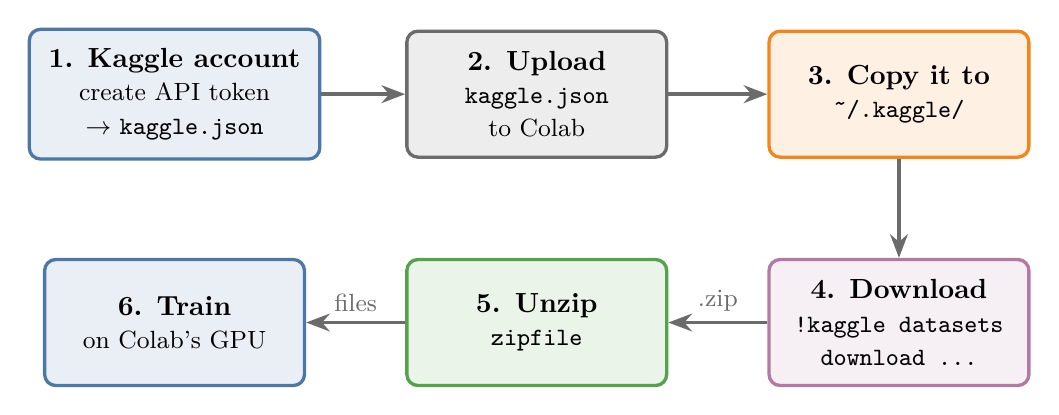
\begin{tikzpicture}
  \node[box=cblue, minimum width=3.3cm, minimum height=1.6cm] (k) at (0,0) {\textbf{1. Kaggle account}\\{\small create API token}\\{\small $\rightarrow$ \texttt{kaggle.json}}};
  \node[box=cgrey, minimum width=3.3cm, minimum height=1.6cm] (u) at (4.6,0) {\textbf{2. Upload}\\{\small \texttt{kaggle.json}}\\{\small to Colab}};
  \node[box=corange, minimum width=3.3cm, minimum height=1.6cm] (c) at (9.2,0) {\textbf{3. Copy it to}\\{\small \texttt{\textasciitilde/.kaggle/}}};
  \node[box=cpurple, minimum width=3.3cm, minimum height=1.6cm] (d) at (9.2,-2.9) {\textbf{4. Download}\\{\small \texttt{!kaggle datasets}}\\{\small \texttt{download \dots}}};
  \node[box=cgreen, minimum width=3.3cm, minimum height=1.6cm] (z) at (4.6,-2.9) {\textbf{5. Unzip}\\{\small \texttt{zipfile}}};
  \node[box=cblue, minimum width=3.3cm, minimum height=1.6cm] (g) at (0,-2.9) {\textbf{6. Train}\\{\small on Colab's GPU}};
  \draw[arrow] (k) -- (u);
  \draw[arrow] (u) -- (c);
  \draw[arrow] (c) -- (d);
  \draw[arrow] (d) -- node[note, above] {.zip} (z);
  \draw[arrow] (z) -- node[note, above] {files} (g);
\end{tikzpicture}
\end{document}
